\chapter{Ejemplos Sencillos}

En este capítulo se van a estudiar la función $\zeta _A (s)$ y la energía de vacío del operador $A = - \partial ^2 _x$, en el intervalo $[0,L]$, sometido a 4 condiciones de contorno. 

En los tres primeros operadores se tomarán condiciones de contorno Dirichlet, Neumann y Periódicas en ambos extremos, luego conociendo sus autovalores  se calculara la función $ \zeta _A (s) $ exactamente. 

En el último operador, se tomará una condición de contorno Dirichlet en un borde y Robin en el otro, luego se utilizarán 3 técnicas distintas para obtener aproximaciones $\zeta _A (s)$: el desarrollo asintótico de los autavalores, una representacion en el plano complejo  y el Heat-Kernel.

\section{Dirichlet,Neumann y Periódicas}

En esta sección estudiará el espectro y las energías de vacío del operador $A = - \partial ^2 _x$ en el intervalo $[0,L]$, al aplicarle condiciones de contorno Dirichlet,Neumann y Periódicas:\\

\textbf{Dirichlet:}


El operador $A$ está dado por:

\begin{equation}
\begin{aligned}
	A \phi (x) &= - \partial _x ^2 \phi (x) \\[10pt]
    \phi (0) &= \phi(L) = 0 
\end{aligned}
\end{equation}



cuyos autovalores y autofunciones son: 

\begin{equation}
\begin{aligned}
	\phi _n (x) &= \sqrt{\frac{2}{L}} \sin( \frac{n \pi x}{L} ) \\[10pt]
	\lambda _n ^2 &= \left( \frac{n \pi }{L} \right) ^2 \\[10pt]
	n &= 1,2,3, ...
\end{aligned}
\end{equation}

la función $\zeta _A (s)$ queda determinada por:

\begin{equation}
\begin{aligned}
\zeta _A (s) &= 
\sum _{n=1} ^{\infty} \left( \frac{\lambda _n}{\mu} \right) ^{-2s}  \\[10pt]
&= \left(  \frac{\pi}{L \mu} \right) ^{-2s}   \sum _{n=1} ^{\infty} n ^{-2s} = 
\left( \frac{\pi}{L \mu} \right) ^{-2s}  \zeta (2s) \\[10pt]
\end{aligned}
\end{equation}


la cual es regular en $s=-1/2$, siendo entonces la energía de vacío:

\begin{equation}
\begin{array}{c}
E _0 = - \frac{\pi}{12 L} \\[8pt]
\end{array}
\end{equation}

lo cual conduce a una fuerza de vacío atractiva. Notar que aquí la constante $\mu$ no parece en el resultado final, esto se debe a que la energía de vacío es finita.\\

\textbf{Neumann:}

El operador $A$ está dado por:

\begin{equation}
\begin{aligned}
	A \phi (x) &= - \partial _x ^2 \phi (x) \\[10pt]
    \phi ' (0) &= \phi ' (L) = 0 
\end{aligned}
\end{equation}



cuyos autovalores y autofunciones están dados por  : 

\begin{equation}
\begin{aligned}
	\phi _0 (x) &= \sqrt{ \frac{1}{L} } \\[5pt]
	\phi _n (x)  &= \sqrt{\frac{2}{L}} \cos \left( \frac{n \pi x}{L} \right) \\[5pt]
	\lambda _n ^2 &= \left( \frac{n \pi }{L} \right) ^2 \\[5pt]
	n &= 1,2,3, ...
\end{aligned}
\end{equation}



la función $\zeta _A (s)$ será la misma que la calculada anteriormente (debido a que se excluyen los modos cero), así como también la energía de vacío. \\

\textbf{Periódicas:}

El operador $A$ está dado por:

\begin{equation}
\begin{array}{c}
	A \phi (x) = - \partial _x ^2 \phi (x) \\[5pt]
    \phi (0) = \phi (L)  \\[5pt]
    \phi ' (0) = \phi ' (L)
\end{array}
\end{equation}

cuyos autovalores y autofunciones están dados por  : 

\begin{equation}
\begin{aligned}
	\phi _{0} &= \sqrt{\frac{1}{L}} \\[5pt]
	\phi _{n} (x) &= \sqrt{\frac{2}{L}} \cos \left( \frac{2 n \pi x}{L} \right) \\[5pt]
	\lambda _n ^2 &= \left( \frac{2 n \pi }{L} \right) ^2 \\[5pt]
	n &= 1,2,3, ...
\end{aligned}
\end{equation}

la función $\zeta _A (s)$ queda determinada por:

\begin{equation}
\begin{aligned}
\zeta _A (s) &= 
\sum _{n=0} ^{\infty} \left( \frac{\lambda}{\mu} \right)^{-2s} \\[5pt]
&=  \left( \frac{2 \pi}{L} \right) ^{-2s} \mu ^{2s} \sum _{n=1} ^{\infty} n ^{-2s} =  
\mu ^{2s} \left( \frac{2 \pi}{L} \right) ^{-2s} \zeta (2s)
\end{aligned}
\end{equation}

que al igual que en los casos anteriores es regular en $s=-1/2$, obteniendo entonces para la Energía de Vacío:

\begin{equation}
E _0 = - \frac{\pi}{6 L}
\end{equation}

lo cual nuevamente conduce a una Energía de Vacío atractiva.

\section{Condiciones de Contorno Mixtas}

En este caso el operador va a depender de un parámetro arbitrario $\gamma$, el cual va a estar dado por:

\begin{equation}
\begin{aligned}
    A \phi (x) &= - \partial ^2 _x \ \phi (x)  \\[5pt]
    \phi (0) &= 0 \\[5pt]
    \phi ' (L) + \gamma \phi (L) &= 0
\end{aligned}
\end{equation}

el cual posee autofunciones de la forma:

\begin{equation}
\phi _n (x) = 
B _n \sin ( \lambda _n x )
\end{equation}

el espectro autovalores $\lambda _n > 0 $ está dado por  cualquiera de las dos ecuaciones equivalentes: 

\begin{equation}
\begin{aligned}
    \frac{\lambda}{\gamma}  \ \cos( L \lambda ) +   \sin( L \lambda ) &= 0 \\[5pt]
    \frac{\lambda}{\gamma}  + \tan (\lambda L )  &= 0 
\label{autovalores}
\end{aligned}
\end{equation}



una vez obtenidos los autovalores el siguiente paso es calcular la función $\zeta _A (s) $ definida por:

\begin{equation}
    \zeta _ {A } (s) = \mu ^{2s} \sum_{n = 1} ^{ \infty } \lambda _n ^ {-2 s}
\end{equation}

al no poder encontrar explícitamente los autovalores se van a utilizar 3 técnicas distintas para estudiar $\zeta _A (s)$.

\subsection{Calculo Asintótico de los autovalores}


Haciendo el cambio a variables adimensionales $\tau = \lambda L $ y $\theta = \gamma L $, las ecuaciones (\ref{autovalores}) se pueden expresar de la forma:

\begin{equation}
\begin{array}{c}
    \tan (\tau) + \frac{\tau}{\theta} = 0 \\[5pt]
    \frac{\tau}{\theta} \cos( \tau ) + \sin( \tau ) = 0
\end{array}
\label{eq.asintota}
\end{equation}

Tal como se puede ver en la figura [\ref{fig:Dibujo1}], los autovalores $\tau _n$ tienden a pegarse a la asíntota vertical de $ \tan ( \tau ) $ a medida que $\tau _n$ crece, por lo tanto los autovalores $\tau _n$ se pueden descomponer en una parte correspondiente a las asíntotas verticales de $ \tan ( \tau )$ mas una corrección que tiende a cero en el límite $ n  \rightarrow \infty$ :

\begin{figure}
    \centering
    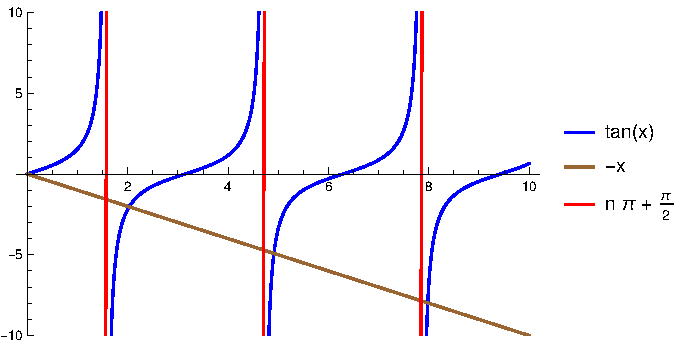
\includegraphics[scale=0.6]{Dibujo.pdf}
    \caption{En este ejemplo, se puede ver que la intersección entre $Tan(x)$ y $-x$ tiende a las asíntotas verticales de la tangente, el mismo comportamiento se aprecia para cualquier recta de la forma $- a x$.}
    \label{fig:Dibujo1}
\end{figure}

\begin{equation}
\begin{array}{c}
    \tau _n = n \pi + \frac{\pi}{2} + \epsilon _n \\[5pt]
    \lim \limits_{ n \rightarrow \infty} \epsilon _n = 0 \\
    
\end{array}
\label{eq.mu}
\end{equation}


Conocer $\epsilon _n $ es equivalente a resolver la ecuación (\ref{eq.asintota}), la cual no posee solución analítica, en vez de eso se va a obtener un desarrollo de $\epsilon _n $ para $n \rightarrow \infty$.

Utilizando (\ref{eq.mu}) en la segunda ecuación de (\ref{eq.asintota}) y desarrollando alrededor de $\epsilon \rightarrow{0}$ se obtiene:

\begin{equation}
\begin{aligned}
    \sin( n \pi + \frac{\pi}{2} + \epsilon _n ) &= 
    - \frac{n \pi + \frac{\pi}{2} + \epsilon _n}{\theta}  \ \cos( n \pi + \frac{\pi}{2} + \epsilon _n )  \\
         (-1) ^n \sum _{p=0} ^{\infty} \frac{(-1) ^p  \epsilon _n ^{2 p }}{(2p)!} 
    &=  \frac{-(n \pi + \frac{\pi}{2} + \epsilon _n) }{\theta}  \  \	
    (-1) ^n
     \sum _{p=0} ^{\infty} \frac{(-1) ^ {p+1} \epsilon _n ^{2 p + 1}}{(2p+1)!} 
\end{aligned}
\end{equation}


Donde reacomodando se llega a la igualdad:

\begin{equation}
    1 = 
    \sum _{p=0} ^{\infty} (-1) ^p     \left[
   	\epsilon _n ^{2p+2 }\left( \frac{1}{(2p+1)! \theta } + \frac{1}{(2p+2)} \right) +
  	\frac{n \pi + \frac{\pi}{2}}{\theta} \frac{  \epsilon _n ^{2p+1}}{(2p+1)!} 			\right]
\label{igualdad epsilon}
\end{equation}

Aquí se puede ver que  $\epsilon _n $ posee un desarrollo en serie de la forma:

\begin{equation}
    \epsilon _n = 
    \frac{\epsilon ^{(1)}}{n}  + 
    \frac{\epsilon ^{(2)}}{n ^2}  + 
    \frac{\epsilon ^{(3)}}{n ^3}  + ...
\label{eq.epsilon}
\end{equation}


Reemplazando este desarrollo de $\epsilon _n$ en (\ref{igualdad epsilon}), e igualando orden a orden se obtiene para los dos primeros ordenes:

\begin{equation}
    \epsilon _n = \frac{\theta}{n \pi} 
     - \frac{ \theta}{2 \pi n ^2 } + O \left( \frac{1}{n ^3}\right) 
\label{epsilons}
\end{equation}

\newpage


La función $ \zeta _A (s)$ queda expresada a este orden como:
    
\begin{equation}
\begin{aligned}
    \zeta _{A} (s) &=  
    \sum _{n=1} ^{\infty} 
    \left( \frac{\lambda _n }{\mu} 
    	\right) ^ {-2 s}  =
    \sum _{n=1} ^{\infty} 
    \left(
	\frac{n \pi}{L \mu} + 
    \frac{\pi}{2 L \mu} +
    \frac{\gamma}{n \pi \mu } -
    \frac{\gamma}{2 n ^2 \pi \mu } +
    O \left(  \frac{1}{n^3} \right) 
    \right) ^{-2 s}  \\[5pt]
    &= \left( \frac{L \mu }{\pi} \right) ^{2s}    
    \sum _{n=1} ^{\infty} 
    n ^{- 2 s} 
    \left(
    1 +     
    \underbrace{
        \frac{1}{2 n} + 
        \frac{L \gamma}{n^2 \pi ^2} -
        \frac{L \gamma}{2 n ^3 \pi ^2} +
        O \left( \frac{1}{n ^{4}} \right) } _{ \chi _n}
    \right ) ^{-2 s}
\end{aligned}
\end{equation}

Para calcular esta serie se desarrolla el binomio alrededor de $\chi _n \rightarrow{0} $ hasta el orden cubico, dado que  cada termino $\chi _{n} ^{m} $ contribuye al orden mas bajo en una potencia $\frac{1}{n ^m}$ .


\begin{align}
\zeta _{A} (s) &= 
\left( \frac{L \mu }{\pi} \right) ^{2s}
\sum _{n=1} ^{\infty}
  n  ^{-2 S} . \\[5pt]
& \ \  \ \Bigg(
	1 - 
	2 s \chi _n +  s(2s+1) \frac{\chi _n ^2}{2} - 
	\frac{2}{3} s(2s+1)(s+1) \chi _n ^3  + O \left( \frac{1}{n ^4} \right) \Bigg)
	\nonumber
\end{align}

Calculadas todas las sumatorias, el resultado final es:





\begin{equation}
\begin{aligned}
    \zeta _A (s) &= \left( \frac{L \mu }{\pi} \right) ^{2s} . \\[5pt]
	& \Bigg(
		\zeta ( 2 s ) -
		s \zeta ( 2s+1 ) +
		 \zeta (2s +2 ) s \left( \frac{1}{4} + \frac{s}{2} - \frac{2 L  \gamma}{\pi ^2} \right)  \\[5pt]
		 & - \zeta (2s+3) \left(  
							\frac{s(s+1) ( \pi ^2 + 2 \pi ^2 s - 24 L \gamma)}{12 \pi ^2 }
		 					\right) 
		+ ...
		\Bigg)
\end{aligned}
\end{equation}


Los polos de $\zeta _A (s)$ están dados por los polos de las funciones $\zeta (s+n)$, desarrollando en los primeros polos se obtiene:

\begin{equation}
\begin{aligned}
\zeta _A (s \rightarrow 1/2) &= 
\frac{L \mu }{2 \pi } \frac{1}{s-1/2} + \ {\rm finito} \\[5pt]
\zeta _A (s \rightarrow 0) &= \ {\rm finito} \\[5pt]
\zeta _A (s \rightarrow -1/2) &= \frac{\gamma}{2 \pi \mu } \frac{1}{s+1/2} 
	+ {\rm finito}\\[5pt]
\zeta _A (s \rightarrow -1) &=  {\rm finito} \\[5pt]
\end{aligned}
\end{equation}

Lo cual está de acuerdo con \ref{eq.ceros.zeta}.

\subsection{Calculo de la función zeta mediante calculo complejo:}

Conocida la ecuación de autovalores, se puede proceder a calcular la función $\zeta _A (s) $ sin calcular explícitamente los autovalores.

Si los  autovalores están definidos por una función $f(\lambda ) = 0$ de la cual son ceros simples, entonces la función $f'(z) / f(z) $ va a tener polos simples en los autovalores de $A$, así la  función $\zeta _A (s)$ va a poder representarse como una integral en el plano complejo, donde el camino de integración es cualquiera de los dos caminos representados en la figura [\ref{fig:contorno}]:

\begin{equation}
\begin{aligned}
   \zeta _A (s) &=  \sum _{n=1} ^{\infty} \left( \frac{\lambda _n}{\mu} \right) ^{-2s} \\[5pt] &=  
   \frac{1}{2 \pi i} \int _{C} \frac{f'(z)}{f(z)} \left( \frac{z}{\mu} \right) ^{-2s} dz 
   =  \frac{1}{2 \pi i} \int _{C} \partial _z \log f(z) \ 
	   \left( \frac{z}{\mu} \right) ^{-2s}
\end{aligned}
\label{asd}
\end{equation}

Reemplazando $f(z)$ por  \ref{autovalores} se obtiene:

\begin{equation}
	\zeta _A (s) = 
    \frac{1}{2 \pi i} \int _{C}
    \frac{ \cos (L z) \left(L + \frac{1}{\gamma} \right) - \sin(L z) \frac{z L}{\gamma}
    }
    { \cos(L z) \frac{z}{\gamma} + \sin(L z)
    }
    \left( \frac{z}{\mu} \right) ^{-2 s} dz
\end{equation}


\begin{figure}
\centering
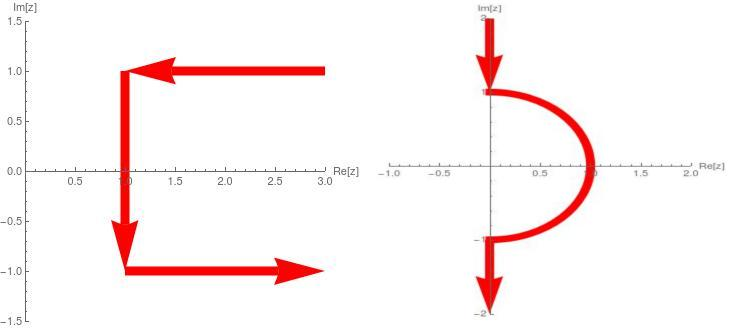
\includegraphics[scale=0.3]{contorno.jpg}
\caption{Camino tenido en cuenta para realizar la integral de contorno en el plano complejo}
\label{fig:contorno}
\end{figure}




Se va a utilizar el camino de la derecha de [\ref{fig:contorno}], el cual se puede descomponer en 3 integrales, una angular y dos rectas, la contribución angular es regular para $ \forall s$, por lo tanto no aporta a la estructura de polos, en cuanto a las contribuciones sobre los ejes se va a parametrizar de la forma $z = \pm i  t$. \\ 


	Luego de tirar los términos exponencialmente decrecientes, los cuales no contribuyen a los polos se obtiene:

\begin{equation}
	\zeta _A (s) = 
    \frac{ \sin (\pi s)}{ \pi } 
    \int _1 ^{\infty} 
    \left( \frac{t}{\mu}  \right)^{-2s}
    \left(
    	L + 
	    \underbrace
    	{
		\frac{1}{\gamma + t}   
		} _{\chi} 
	\right)
    dt 
\label{contorno}
\end{equation}

Donde en el denominador se puede calcular factor común $t$ y utilizar la serie geométrica para obtener:

\begin{equation}
    \chi =   \sum _{m=0} ^{\infty} \frac{(-1) ^{m} \gamma ^{m} }{t ^{m+1}}
\label{eq:chi}
\end{equation}

Luego de integrar termino a termino, el resultado final es:

\begin{equation}
    \zeta _A (s) = 
    \frac{ \sin(\pi s) \mu ^{2s }}{\pi } 
    \left(
    \frac{L}{2s-1} + 
    \sum _{m=0} ^{\infty}
    \frac{(-1) ^{m} \gamma ^{m} }{2s+m}
    \right)
\label{eq.zeta.com}
\end{equation}

De aquí se puede ver que la función $\zeta _A (s)$ tiene polos simples en $s=1/2$ y los semienteros negativos, la estructura de polos queda determinada por:

\begin{equation}
\begin{aligned}
\zeta(s \rightarrow 1/2) &= \frac{L \mu }{2 \pi} \frac{1}{s-1/2} + finito \\
\zeta (s \rightarrow -n - 1/2)  &= \frac{ (-1) ^n \gamma ^{2n+1}  }{2 \pi \mu ^{2n + 1}} \frac{1}{s + n + 1/2} + finito
\end{aligned}
\end{equation}


El cual coincide a los primeros orden con lo calculado en la sección anterior  y a todos los ordenes con (\ref{eq.ceros.zeta}).

 Utilizando esta técnica se puede sacar la estructura entera de polos de la función $\zeta _A (s) $, pero sin calcular la parte finita de estas expresiones, para calcular la parte finita hay que tener en cuenta la parte angular de (\ref{asd}), y los términos exponenciales tirados para llegar a (\ref{contorno}).


\subsection{Uso del Heat-Kernel:}


Utilizando la formula (\ref{losresi}), luego de calcular los coeficientes del Heat Kernel dados por \cite{VASSILEVICH2003279}, se obtiene:



\begin{equation}
\begin{aligned}
Res \  \zeta _A (s)  | _{s=1/2} &= \frac{L \mu}{2 \pi} \\[5pt]
Res \  \zeta _A (s)  | _{s=0} &= 0 \\[5pt]
Res \ \zeta _A (s) | _{s=-1/2} &= \frac{\gamma}{2 \pi \mu} \\[5pt]
Res \  \zeta _A (s) | _{s=-1} &= 0 \\[5pt]
\end{aligned}
\end{equation}


Lo cual, también coincide con los dos métodos anteriores y (\ref{eq.ceros.zeta}).
